\documentclass[12pt]{article}
\usepackage{booktabs}
\usepackage[utf8]{inputenc}
\usepackage{multicol, graphicx}
\graphicspath{ {Images/} }
\pagestyle{empty}
\usepackage{amsfonts,amsmath}
\usepackage{tikz}
\newcommand{\mycbox}[1]{\tikz{\path[draw=#1,fill=#1] (0,0) rectangle (.2cm,.2cm);}}
\usepackage{amsmath}
\usepackage{amssymb}
\newtheorem{theorem}{THEOREM}
\newtheorem{proof}{PROOF}


\usepackage{float}
\usepackage{caption}
\usepackage{subcaption}
\addtolength{\oddsidemargin}{-.875in}
\addtolength{\evensidemargin}{-.875in}
\addtolength{\textwidth}{1.75in}
\addtolength{\topmargin}{-.875in}
\addtolength{\textheight}{1.75in}




















\def\Rl{\mathbb{R}}


\begin{document}

\centerline{{\sc Problem Set No. 3(Last Problem Set)}}
\bigskip
\centerline{CS 297 - Dynamical System}
\centerline{by: Bel, Joshua and Racquel}

%\begin{theorem}
%Trial theorem package
%\end{theorem}
\bigskip\noindent
{\bf EXERCISES FOR CHAPTER 7 }\\
{\bf 7.1.8 A Circular Limit Cycle} \\
Consider $\ddot{x} + a\dot{x}(x^2+\dot{x}^2-1)+x = 0$, where $a > 0$.
\\{\bf Solution: }\\
\indent
{\bf a. }\\ 

Let $\begin{cases} \dot{x}=y \\ \dot{y}=-ay(x^2 + y^2 -1) -x \end{cases}$ . \\

To let $\dot{x}=0$, we get $y = 0$. Substituting this in the second equation, we get $(\dot{x},\dot{y} = (0,0)$ when $(x,y) = (0,0)$. Thus the origin is a fixed point.Taking the Jacobian, \\
\begin{align*}
J&=\begin{bmatrix}
0 & 1\\
-2axy & -1
\end{bmatrix}\\
&= \begin{bmatrix}
0 & 1\\
-1 & a
\end{bmatrix},\text{at the origin}\\
(-\lambda)(a-\lambda) + 1 &= 0\\
\lambda^2 -a\lambda + 1 &=0\\
\lambda &= \frac{a \pm \sqrt[]{a^2-4}}{2}
\end{align*}
Note that $a > 0$. Then if $0 < a < 2$, the roots are complex conjugates, the fixed point is an unstable spiral. If $a > 2$, the roots are positive, then the fixed point is an unstable node.\\

{\bf b. }Expressing the equations in polar coordinates:\\
\begin{align*}
r\dot{r} &= x\dot{x} + y\dot{y}\\
&=xy + y(-ay(x^2 + y^2 -1) - x)\\
&=-ay^2(x^2 + y^2 -1)\\
&=-ar^2sin^2\theta (r^2 - 1)\\
\dot{r} &= -arsin^2\theta(r^2 - 1)
\end{align*}
Also,
\begin{align*}
\dot{\theta} &= \frac{x\dot{y} - y\dot{x}}{r^2}\\
&= \frac{x(-ay(x^2 + y^2 -1) -x) - y^2}{r^2}\\
&= \frac{-(x^2+y^2) -axy(x^2 + y^2 -1)}{r^2}\\
&= \frac{-r^2 -ar^2sin\theta cos\theta (r^2-1)}{r^2}\\
&= -1 -asin\theta cos\theta (r^2 - 1)
\end{align*}
At $\dot{r}=0$ , since $r \geq 0$, either $r=0$ or $r=1$. At $r=1$, $\dot{\theta} = -1$.
Then there exists a circular limit cycle with amplitude 1 and period $2\pi$.\\

{\bf c. }Since $f(r,\theta) = -arsin^2\theta(r^2 -1 )$,\\
\begin{align*}
\frac{\partial f}{\partial r} &= -asin^2\theta(3r^2-1)\\
&=-2asin^2\theta, \text{at r=1}\\
&\leq 0, \text{stable.}
\end{align*}

{\bf d. }From part b, it was seen that if $\dot{r}=0$, either $r=0$ or $r=1$. Then the only other choice for a limit cycle is when $r=0$. If r, the amplitude, is zero, this reduces to a point, and there is no limit cycle to speak of. Thus the cycle $r=1$, $\dot{\theta} = -1$ is unique.\\

\noindent
{\bf 7.2.10 Liapunov Function} \\
{bf Solution: }\\
Let
\begin{align*}
V &=ax^2+by^2\\
\dot{V} &=2ax\dot{x}+2by \dot{y}\\
&= 2ax(y=x^3)+2by(-x-y^3)\\
&=(2a-2b)xy-2ax^4-2by^4
\end{align*}
Now, if $a=b$ then the $xy$ term vanishes then any value of $a$ can do, say take $\frac{1}{2}. \Rightarrow V=\frac{1}{2}(x^2+y^2) \Rightarrow \dot{V}=-(x^4+y^4)<0$ for all $x,y$ not equal to zero and $V$ is positive. This implies that there cannot be any closed orbits in this system.\\

{\bf 7.2.13 Dulac and Competition Model}\\
{\bf Solution:} \\
Let 
\begin{align*}
g &=\frac{1}{N_1 N_2},~~~ N=(N_1, N_2)~\text{such that}~\\ \dot{N_1} &=r_1 N_1(1-\frac{N_1}{K_1})-b_1N_1N_2,\\
\dot{N_2} &=r_2 N_2(1-\frac{N_2}{K_2})-b_2N_1N_2\\
\nabla \cdot \left(g \dot{N}\right)&=\frac{\partial}{\partial N_1}\left(g \cdot \dot{N_1}\right)+\frac{\partial}{\partial N_2}\left(g \cdot \dot{N_2}\right)\\
&=\frac{\partial}{\partial N_1}\left(\frac{r_1}{N_2}\left(1-\frac{N_1}{K_1}-b_1\right)\right)+\frac{\partial}{\partial N_2}\left(\frac{r_2}{N_1}\left(1-\frac{N_2}{K_2}-b_2\right)\right)\\
&=-\frac{r_1}{K_1 N_2}-\frac{r_2}{K_2 N_1}\\
\end{align*}
Since $r_1,r_2, K_1,K_2$ are all positive parameters, $N_1, N_2 >0.$\\
$\therefore \nabla \cdot \left(g \dot{N} \right)<0.$\\
Now, by Dulac's criterion implies that there are no closed orbits in the first quadrant. \mycbox{black}\\
{\bf 7.3.4 Poincare-Bendixson}\\
Consider the system
$\begin{cases}
\dot{x} = x(1-4x^2 - y^2) - \frac{1}{2}y(1+x)\\
\dot{y} = y(1-4x^2 -y^2) +2x(1+x)
\end{cases}$.\\
{\bf Solution:}\\
\indent
{\bf a. } The Jacobian,
\begin{align*}
J&=\begin{bmatrix}
1-12x^2-y-\frac{1}{2}y & -2xy - \frac{1}{2} -\frac{1}{2}x\\
-8xy +2 + 4x& -1 - 4x^2 - 3y^2
\end{bmatrix}. \\
&=\begin{bmatrix}
1 & - \frac{1}{2}\\
2 & -1 
\end{bmatrix}, \text{at the origin}
\end{align*}
Taking the eigenvalues, 
\begin{align*}
(1-\lambda)^2 + 1 &=0\\
\lambda^2 -2\lambda + 2 &=0\\
\lambda &= \frac{2 \pm \sqrt{4-8}}{2}\\
&= 1\pm i
\end{align*}.
Since the eigenvalues are complex conjugates, the origin is an unstable spiral.\\
\indent
{\bf b. } Let $V = (1-4x^2 -y^2)^2$. Then
\begin{align*}
\dot{V} &= 2(1-4x^2-y^2)(-8x\dot{x}-2y\dot{y})\\
&=2(1-4x^2-y^2)(-8x(x(1-4x^2 - y^2) - \frac{1}{2}y(1+x))-2y(y(1-4x^2 -y^2) +2x(1+x)))\\
&=2\sqrt{V}(-8x^2\sqrt{V}+4xy(1+x) -2y^2\sqrt{V} - 4xy(1+x))\\
&=-4\sqrt{V}(4x^2\sqrt{V}+y^2\sqrt{V})\\
&=-4V(4x^2 + y^2)\\
& \leq 0, \text{since } V,x^2, y^2 \geq 0
\end{align*}
Since $V\geq 0$ and is decreasing, then $\lim_{t \to \infty} V = 0$.
\\Thus, all trajectories approach the ellipse $4x^2 + y^2 = 1$ as $t\to\infty$.\\


\bigskip\noindent
{\bf 7.4.2 Lienard System} \\
{\bf Solution:} \\
{\bf 7.5.6 Biased Van der Pol} \\
{\bf Solution:}\\
\indent
{\bf a. } To classify all the fixed points, we first write out our system in Lienard form. First we define $F(x)$ so that
\begin{align*}
\ddot{x}+\mu(x^2-1)\dot{x}=\frac{d}{dx}\left(\dot{x}+\mu F(x)\right),
\end{align*}
which works out if $F(x)=\frac{x^3}{3}-x,$  just as it did in the non-biased case. Now, we find that $\dot{y}=-\frac{(x-a)}{\mu}.$ Thus, our system becomes
\begin{align*}
\dot{x} &=\mu[y-F(x)]\\
\dot{y} &=-\frac{x-a}{\mu}
\end{align*}
Thus, our $x-$ nullcline becomes $y=F(x)$ and our $y-$ nullcline becomes $x=a.$ The intersection and the only fixed point is at $x^*=\left(a,F(a)\right)=\left(a,a^3/3-a\right).$ Next, we compute the Jacobian matrix and evaluate at $X^*.$

\begin{figure}[htp]
  \centering
  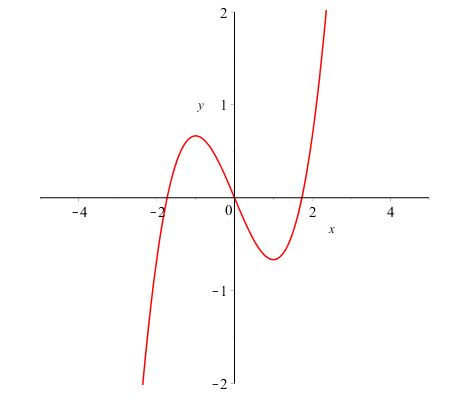
\includegraphics[width=4cm]{7_5_6_a}
  \caption{}
\end{figure}

Now,\\
\begin{align*}
J&=\left(\begin{array}{cc} -\mu (x^2-1) & \mu \\
-\frac{1}{\mu} & 0
\end{array}\right).
\end{align*}
From this we find that our trace and determinant are going to be given by $T=\mu(a^2-1)$ and $D=1.$  Furthermore, we have that the system is unstable when $-1< a <1$ and unstable otherwise. Moreover, for sufficiently high values of $a$ the value of $T^2-4D=\mu^2(a^2-1)^2-4$ will be positive, implying that the fixed point will be a node. Clearly, this can't always be the case, since plugging in $a=1$ readily checks out as giving us negative value for $T^2-4D,$ implying that we do have spiral behaviour for certain values of $a.$\\
\indent
{\bf b. } See figure below for a numerically produced plot given that $a=0.4$ and $\mu=5,$ which has been laid on top of a vector field of that system. Now, to see that the fixed point in cases like these are unstable, we resort to the work we did for part $(a)$ with respect to finding stabilities of fixed points for various regions.\\
\indent
{\bf c. } In this case, for $|a|<a_c=1,$ the $y-$ nullcline intersects the $x-$ nullcline on the middle branch of the cubic nullcline. We know that when this is the case the intersection, the fixed point, is unstable, so all initial conditions move away from that point. Furthermore, they all move toward the cubic nullcline, and once there, they will move up along the nullcline if it has reached the negative leg, and will move down if on the positive leg. Eventually, the trajectory will reach either a local maximum or local minimum depending on which leg you are on.

\begin{figure}[htp]
  \centering
  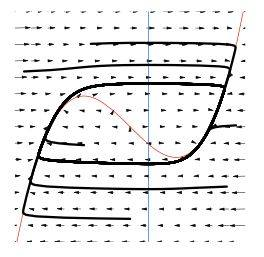
\includegraphics[width=4cm]{7_5_6_c}
  \caption{}
\end{figure}

Now, if $|a|>a_c,$ there can be no stable limit cycle, since the $x$ nullcline intersects the cubic nullcline along one of the positive branches, and consequently, once a trajectory hits that nullcline, it will move slowly along it and toward the intersection since if it hits below the intersection, then $x<a$ so $\dot{x}$ is positive and similarly negative if $x>a.$ Thus, since all trajectories end up moving slowly along nullclines and toward the fixed point, there can be no stable limit cycles.\\
\indent
{\bf d. } Graph:\\

\begin{figure}[htp]
  \centering
  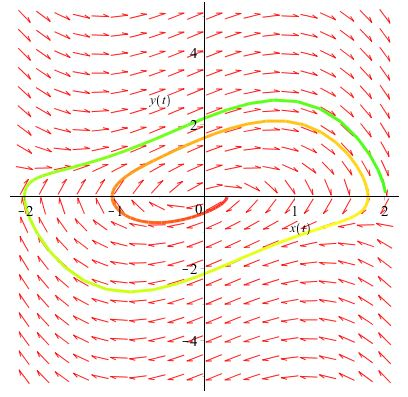
\includegraphics[width=4cm]{7_5_6_d}
  \caption{}
\end{figure}

If if $a=1.1$, all of the trajectories end up getting stuck near the local minimum of the cubic nullcline. Now, if a slight disturbance moves the state of the system to just below the fixed point then it will shoot across to the negative leg of the cubic, and then go along the whole of the cycle but get stuck again at the globally attracting rest state.\\


\noindent
{\bf 7.6.14 Computer Test of Two-Timing}\\

\noindent
{\bf 8.1.10 Budworms in Forest}\\
{\bf Solution:}\\

\bigskip\noindent
{\bf 8.2.10 Bacterial Respiration} \\
{\bf Solution:} \\
\indent
{\bf a. }\\
{\bf 8.3.2 Chemical Oscillator}\\
{\bf Solution:}\\
\indent
{\bf a. } Let 
\begin{align*}
\dot{x}&=a-x+x^2y\\
\dot{y}&=b-x^2y.
\end{align*}
Let us consider $\frac{\dot{y}}{\dot{x}}$ i.e., $\frac{b-x^2y}{a-x+x^2y}.$ Using the figure in letter e below, we have clearly seen that all trajectories eventually enter a certain trapping region, to be determine.\\

\indent
{\bf b. } To show that the system has a unique fixed point, let $\dot{x}=0$ and $\dot{y}=.$ That is\\
\begin{align}
a-x+x^2y=0\\
b-x^2y=0
\end{align}
Now, the second equation is equal to $b=x^2y$. Then substituting this to equation 1, we have $a-x+b=0 \Rightarrow x=a+b.$ Now, if $x=a+b,$ substituting this to equation 2, we have
\begin{align*}
b&=x^2y\\
b&=(a+b)^2y\\
\Rightarrow y=\frac{b}{(a+b)^2}.
\end{align*}
Thus, we only have one solution to the system that is $\left(a+b,\frac{b}{(a+b)^2}\right).$ Hence, the system has a unique fixed point.\mycbox{black}\\
To classify the fixed point, let's analyze the system first by considering its Jacobian matrix. That is 
\begin{align*}
J&=\left(\begin{array}{cc} 2xy-1 & x^2 \\
-2xy & -x^2
\end{array}\right).
\end{align*}
Now, 
\begin{align*}
J\left(a+b,\frac{b}{(a+b)^2}\right)&=\left(\begin{array}{cc} \frac{2b}{a+b}-1 & (a+b)2 \\
-\frac{2b}{a+b} & -(a+b)^2
\end{array}\right).\\ 
\end{align*}
$\Rightarrow$ determinant of $J(\left(a+b,\frac{b}{(a+b)^2}\right)=(a+b)^2$ and trace is $\tau=\frac{2b}{a+b}-1-(a+b)^2.$ Now the fixed point is stable if $det\left(J\left(a+b,\frac{b}{(a+b)^2}\right)\right)=(a+b)^2>0$ and trace $\tau=\frac{2b}{a+b}-1-(a+b)^2<0$.\\
Notice that the determinant is always positive and the trace is negative, that is if $\tau=\frac{2b}{a+b}-1-(a+b)^2<0\Rightarrow b-a<(a+b)^3.$ Hence, it is stable if this condition is satisfied.\\
\indent
{\bf c. } To show that the system undergoes a Hopf bifurcation when $b-a=(a+b)^3,$ let us consider the trace of the system. Now, hopf bifurcation occurs in this system if the trace is zero. That is,
\begin{align*}
\frac{2b}{a+b}-1-(a+b)^2&=0\\
\frac{2b}{a+b}-1&=(a+b)^2\\
2b-(a+b)&=(a+b)^2(a+b)\\
2b-a-b&=(a+b)^3\\
b-a&=(a+b)^3. \mycbox{black}
\end{align*}
\indent
{\bf d. } Now, please refer the diagram in letter e to determine the type of hopf bifurcation.\\

Notice, in figure 1 we have $a=0, b=1$ which are the parameter values. Now, in figure 2, $a=1/2, b=0.9$ we notice that for a small disturbance the equilibrium state slowly loses its stability. This is a supercritical hopf bifurcation.\\
{\bf e. } Stability Diagram in $a$ and $b.$

\begin{figure}[htp]
  \centering
  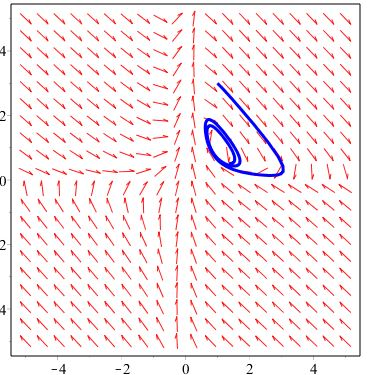
\includegraphics[width=4cm]{8_3_2_d}
  \caption{}
\end{figure}
\begin{figure}[htp]
  \centering
  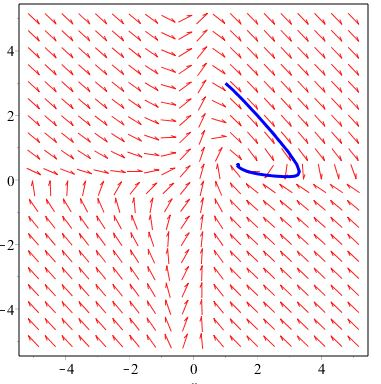
\includegraphics[width=4cm]{8_3_2_d_2}
  \caption{}
\end{figure}

\bigskip\noindent
{\bf 8.4.9 Resonance and Cusp Catastrophy} \\
{\bf Solution:} \\

\noindent
{\bf 8.5.3 Logistic with Periodically varying carrying capacity }\\
{\bf Solution: }\\

\noindent
{\bf 8.6.7 Mechanical Example of Quasi-periodicity}
{\bf Solution:}\\

{\bf a. } Note that if there is a circular motion, there is no change of the radius $\ddot{r=0.}$ Then we can write 
\begin{align*}
m\ddot{r}=0=\frac{h^2}{mr_0^3}-k \Longleftrightarrow r_0=\sqrt[3]{\frac{k^2}{mk}}.
\end{align*}
Then afterwards, the second equation can be arranged as 
\begin{align*}
\dot{\theta}=\omega_0=\frac{h}{mr_0^2}\Longleftrightarrow \omega_0=\sqrt[3]{\frac{k^2}{hm}}.
\end{align*}

\indent
{\bf b. } Now, taking into account the small radial perturbations $r=r_0+\delta r$ gives the equation below
\begin{align*}
m\frac{d^2}{dt^2}\left(r_0+\delta r\right)=\frac{h}{m \left(r_0+\delta r\right)^3}-k.
\end{align*}

\noindent
{\bf 8.7.3 Overdamped System with square-wave forcing } 
{\bf Solution} \\

\noindent
{\bf 9.1.4 Laser Models}\\
{\bf Solution: } \\
{\bf a. } To show that the non-lasing state loses stability above a threshold value of $\lambda$, we consider $\dot{P}=0$ which gives $ED=P$ and $\dot{D}=0$ that gives $D=\lambda+1 -\lambda E P.$ Thus,
\begin{align*}
P=\frac{(\lambda+1)E}{\lambda E^2+1}
\end{align*}
and
\begin{align*}
\dot{E}=k\left(\frac{(\lambda+1)E}{\lambda E^2+1}-E\right)
\end{align*}

Now, we let $f(E)=k\left(\frac{(\lambda+1)E}{\lambda E^2+1}-E\right)$ and $f'(E)=k\left[\frac{(\lambda+1)\left(1-\lambda E^2\right)}{\left(\lambda E^2+1\right)^2}-1\right]$\\
We take note of the following cases.\\
\begin{itemize}
\item[1.] If $\lambda <0,$ there are 3 fixed points $E_1^*=0, E_2^*=1$ and $E_3^*=-1.$ The derivative at $E_1^*=0$ is $f'(E_1^*)=\lambda k,$ so it is stable.\\
\item[2.] If $\lambda=0,$ there are infinite fixed points. The derivative at $E^*=0$ is $f'(E^*)=0,$ showing that $\lambda=0$ is the bifurcation value.\\
\item[3.] If $\lambda >0,$ there are 3 fixed points $E_1^*=0, E_2^*=1$ and $E_3^*=-1.$ The derivative at $E_1^*=0$ is $f'(E_1^*)=\lambda k>0,$ so it is unstable.
\end{itemize}
Therefore, we have a degenerate pitchfork bifurcation.\\
\indent
{\bf b. } By comparing the equation of $\dot{\tilde{x}}$ and $E,$ we have $\tilde{t}=\frac{kt}{\sigma}, \tilde{x}=\alpha E$ and $\tilde{y}=\alpha P$ where $\alpha$ needs to be determined. Now we have,
\begin{align*}
\frac{d \tilde{x}}{d \tilde{t}}=\frac{\alpha dE}{k/ \sigma dt}=\frac{\alpha \sigma dE}{k dt }=\alpha \sigma (P-E)=\sigma(\tilde{y}-\tilde{x})
\end{align*}
 Then we compute $\frac{d \tilde{y}}{d \tilde{t}}$ with $\dot{P}$ to obtain the transformation of $\gamma_1$ and $D.$
\begin{align*}
\frac{d \tilde{y}}{d \tilde{t}}= \frac{\alpha  \sigma dP}{k dt}=\frac{\alpha \sigma}{k} \gamma_1(ED -P)=\frac{\sigma}{k} \gamma_1(\tilde{x} D-\tilde{y})=\tilde{x}(r-\tilde{z})-\tilde{y}
\end{align*}
Therefore $\gamma_1=\frac{k}{\sigma}$ and $D=r-\tilde{z}.$\\
This time we finally compute $\frac{d \tilde{z}}{d \tilde{t}}$ with $\dot{E}$ to determine the transformation of the remaining variables.\\
\begin{align*}
\frac{d \tilde{z}}{d \tilde{t}}= -\frac{dD}{k/ \sigma dt}=-\frac{\sigma dD}{k dt}=-\frac{\sigma \gamma_2}{k}\left(\lambda +1 -D-\lambda EP\right)=\frac{\sigma \gamma_2}{k}\left(\lambda+1-r \right)-\frac{\sigma \gamma_2}{k}\tilde{z}+\frac{\sigma \gamma_2}{k} \alpha^2 \lambda \tilde{x} \tilde{y}=\tilde{x} \tilde{y}-b \tilde{z}
\end{align*}
Therefore $\lambda=r-1, \gamma_2=\frac{bk}{\sigma}$ with a special relationship $a=[b(r-1)]^{-1/2}.$\\

{\bf 9.2.6 Geometric Reversals} ( The leaky bucket)\\
{\bf Solution:}\\
\indent
{\bf a. } \\

\bigskip\noindent
{\bf 9.3.10 Time Horizon} \\
{\bf Solution:} \\
Here is the graph of the Lorenz equations when $r=28,\sigma=10,b=8/3.$\\

\begin{figure}[htp]
  \centering
  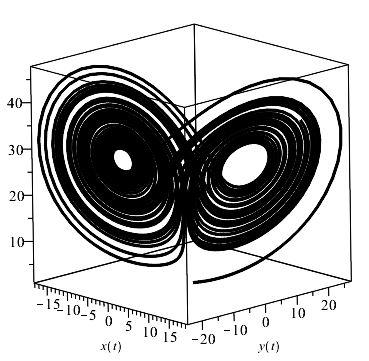
\includegraphics[width=4cm]{9_3_10}
  \caption{}
\end{figure}

\begin{figure}[htp]
  \centering
  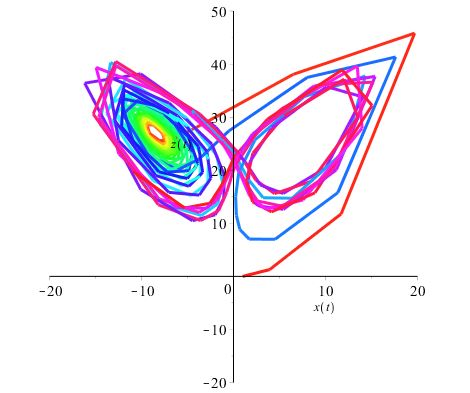
\includegraphics[width=4cm]{9_3_10_xt}
  \caption{}
\end{figure}



{\bf 9.4.2 Tent Map}\\
{\bf Solution:}\\
\indent
{\bf a. } It is called a tent map because the graph of f(x) looks like a triangle with vertices at (0,0), (1,0) and (0,1). Thus, if the x-axis is the ground, then f(x) looks like a tent set-up on it.\\
\indent
{\bf b. } If $0 \leq x \leq \frac{1}{2}$, then $f(x^*) = 2x^* = x^* \rightarrow x^* = 0$. Also, $|f'(x^*)| = |2| > 1$, unstable.\\
\indent 
If $\frac{1}{2} \leq x \leq 1$, then $f(x^*) = 2- 2x^* = x^* \rightarrow x^* = \frac{2}{3}$. Also, $|f'(x^*)| =|- 2| > 1$, unstable.\\
 \indent
{\bf c. }
\begin{table}[h!]
  \centering
  \begin{tabular}{c|c||c|c|c|c|c}
    Case &Conditions & $f(f(x))$ & $x^*$ & Period 2? & $f'(f(x^*))$ & Stability\\
    \hline
    1&$0\leq x \leq \frac{1}{2}, 0\leq f(x) \leq \frac{1}{2}$  & 2(2x) = 4x & 0 & No & & \\
    2&$0\leq x \leq \frac{1}{2}, \frac{1}{2} \leq f(x) \leq 1$  & 2-2(2x) = 2 - 4x & $\frac{2}{5}$ & Yes &-4&Unstable\\
    3&$\frac{1}{2} \leq x \leq 1, 0\leq f(x) \leq \frac{1}{2}$  & 2(2-2x) = 4 - 4x & $\frac{4}{5}$ & Yes &-4&Unstable\\
    4&$\frac{1}{2} \leq x \leq 1, \frac{1}{2} \leq f(x) \leq 1$  & 2-2(2-2x) = -2 + 4x & $\frac{2}{3}$ & No & & \\
  \end{tabular}
\end{table}\\
{\bf d. }To check for Period 3:
\begin{table}[h!]
  \centering
  \begin{tabular}{c|c||c|c|c|c|c}
    Case &Conditions & $f(f(f(x)))$ & $x^*$ & Period 3? & $f'f((f(x^*)))$ & Stability\\
    \hline
    1&Case 1 in c, $0\leq f(f(x)) \leq \frac{1}{2}$  & 2(4x) = 8x & 0 & No & & \\
    2&Case 1 in c, $\frac{1}{2} \leq f(f(x)) \leq 1$  & 2-2(4x) = 2 - 8x & $\frac{2}{9}$ & Yes &-8 & Unstable\\
    3&Case 2 in c, $0\leq f(f(x)) \leq \frac{1}{2}$  & 2(2-4x) = 4 - 8x & $\frac{4}{9}$ & Yes &-8 & Unstable \\
    4&Case 2 in c, $\frac{1}{2} \leq f(f(x)) \leq 1$  & 2-2(2-4x) = -2 + 8x & $\frac{2}{7}$& Yes &8 & Unstable \\
    5&Case 3 in c, $0\leq f(f(x)) \leq \frac{1}{2}$  & 2(4-4x) = 8 - 8x & $\frac{8}{9}$ & Yes &-8 & Unstable \\
    6&Case 3 in c, $\frac{1}{2} \leq f(f(x)) \leq 1$  & 2-2(4-4x) = -6 + 8x & $\frac{6}{7}$ & Yes &8 & Unstable \\
    7&Case 4 in c, $0\leq f(f(x)) \leq \frac{1}{2}$  & 2(-2+4x) = -4 + 8x & $\frac{4}{7}$ & Yes &8 & Unstable \\
    8&Case 4 in c, $\frac{1}{2} \leq f(f(x)) \leq 1$  & 2-2(-2+4x) = 6 - 8x & $\frac{2}{3}$ & No & & \\
  \end{tabular}
\end{table}\\
To check for Period 4:
\begin{table}[h!]
  \centering
  \begin{tabular}{c|c||c|c|c|c|c}
    Case &Conditions & $f(f(f(f(x))))$ & $x^*$ & Period 4? & $f'^4(x^*)$ & Stability\\
    \hline
    1&Case 1 above, $0\leq f(f(f(x))) \leq \frac{1}{2}$  & 2(8x) = 16x & 0 & No & & \\
    2&Case 1 above, $\frac{1}{2} \leq f(f(f(x))) \leq 1$  & 2-2(8x) = 2 - 16x & $\frac{2}{17}$ & Yes &-16 & Unstable\\
    3&Case 2 above, $0\leq f(f(f(x))) \leq \frac{1}{2}$  & 2(2-8x) = 4 - 16x & $\frac{4}{17}$ & Yes &-16 & Unstable \\
    4&Case 2 above, $\frac{1}{2} \leq f(f(f(x))) \leq 1$  & 2-2(2-8x) = -2 + 16x & $\frac{2}{15}$ & Yes &16 & Unstable\\
    5&Case 3 above, $0\leq f(f(f(x))) \leq \frac{1}{2}$  & 2(4-8x) = 8-16x &$\frac{8}{17}$ & Yes &-16 & Unstable \\
    6&Case 3 above, $\frac{1}{2} \leq f(f(f(x))) \leq 1$  & 2-2(4-8x) = -6 + 16x & $\frac{2}{5}$ & No & &\\
    7&Case 4 above, $0\leq f(f(f(x))) \leq \frac{1}{2}$  & 2(-2+8x) = -4 + 16x & $\frac{4}{15}$ & Yes &16 & Unstable\\
    8&Case 4 above, $\frac{1}{2} \leq f(f(f(x))) \leq 1$  & 2-2(-2+8x) = 2 - 16x & $\frac{2}{17}$ & Yes &-16 & Unstable\\
    9&Case 5 above, $0\leq f(f(f(x))) \leq \frac{1}{2}$  & 2(8-8x) = 16 - 16x & $\frac{16}{17}$ & Yes &-16 & Unstable\\
    10&Case 5 above, $\frac{1}{2} \leq f(f(f(x))) \leq 1$  & 2-2(8-8x) = -14 + 16x & $\frac{14}{15}$ & Yes &16 & Unstable\\
    11&Case 6 above, $0\leq f(f(f(x))) \leq \frac{1}{2}$  & 2(-6+8x) = -12 + 16x & $\frac{4}{5}$ & No & & \\
    12&Case 6 above, $\frac{1}{2} \leq f(f(f(x))) \leq 1$  & 2-2(-6+8x) = 10 - 16x & $\frac{10}{17}$ & Yes &-16 & Unstable\\
    13&Case 7 above, $0\leq f(f(f(x))) \leq \frac{1}{2}$  & 2(-4+8x) = -8 + 16x & $\frac{8}{15}$ & Yes &16 & Unstable\\
    14&Case 7 above, $\frac{1}{2} \leq f(f(f(x))) \leq 1$  & 2-2(-4+8x) = 6 - 16x & $\frac{6}{17}$ & Yes &-16 & Unstable\\
    15&Case 8 above, $0\leq f(f(f(x))) \leq \frac{1}{2}$  & 2(6-8x) = 12 - 16x & $\frac{12}{17}$ & Yes &-16 & Unstable\\
    16&Case 8 above, $\frac{1}{2} \leq f(f(f(x))) \leq 1$  & 2-2(6-8x) = -10 + 16x & $\frac{2}{3}$ & No & & \\
  \end{tabular}
\end{table}\\

\bigskip
 \noindent
{\bf 9.5.4 Hysteresis} $\dot{x}=3$\\
{\bf Solution: }\\

\noindent
{\bf 9.6.3 Synchronized Chaos}\\
{\bf Solution: }\\
{\bf a. } Below are the plots for the 3 D graph of the Lorenz Equation and the system associated in exercise 9.6.2 respectively. Then followed by $y(t)$ and $y_r(t).$

\begin{figure}[htp]
  \centering
  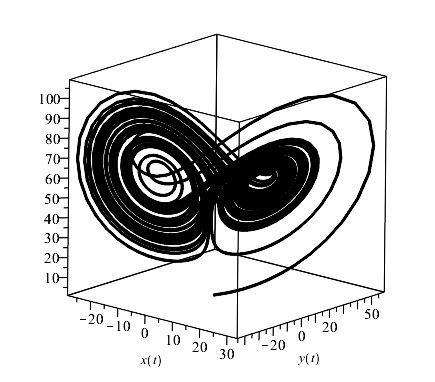
\includegraphics[width=4cm]{9_6_3_xyz}
  \caption{ $r=60, \sigma=10,b=8/3$}
\end{figure}
\begin{figure}[htp]
  \centering
  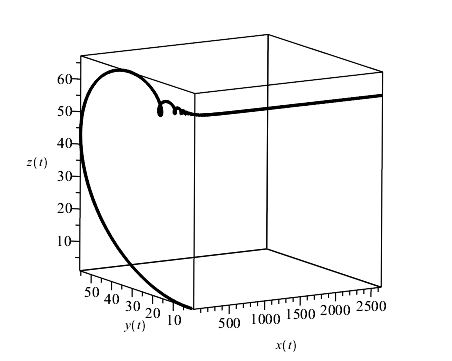
\includegraphics[width=4cm]{9_6_3_xyzr}
  \caption{Graph of the system associated in 9.6.2}
\end{figure}
Here are the graphs of $y(t)$ and $y_r(t).$
\begin{figure}[htp]
  \centering
  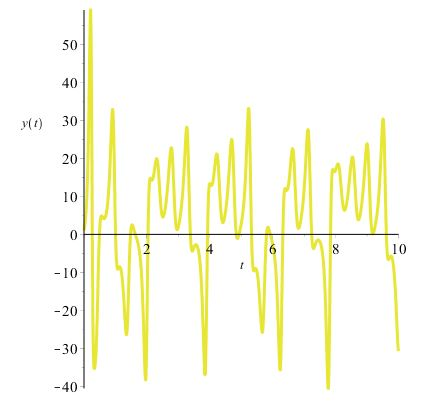
\includegraphics[width=4cm]{9_6_3_a_yt}
  \caption{$y(t)$}
\end{figure}
\begin{figure}[htp]
  \centering
  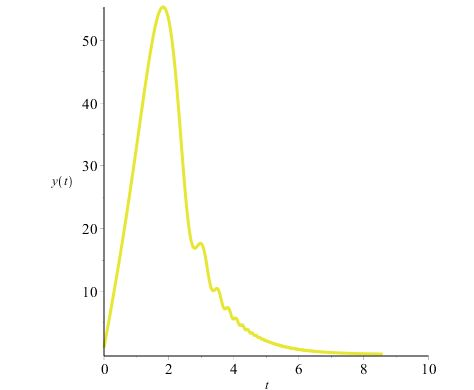
\includegraphics[width=4cm]{9_6_3_a_yrt}
  \caption{$y_r(t)$}
\end{figure}

{\bf b. } Here are the the plot of the projection $(y,z)$ of both trajectories.
\begin{figure}[htp]
  \centering
  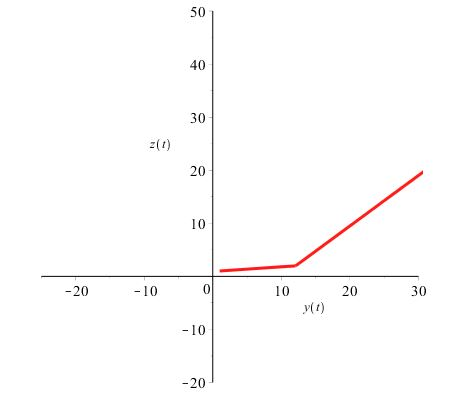
\includegraphics[width=4cm]{9_6_3_b_projyt}
  \caption{$y(t)$}
\end{figure}
\begin{figure}[htp]
  \centering
  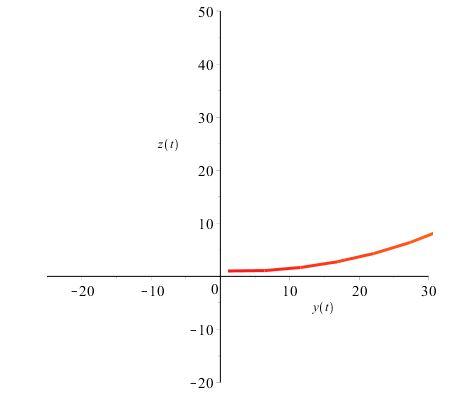
\includegraphics[width=4cm]{9_6_3_b_projyrt}
  \caption{$y_r(t)$}
\end{figure}

\pagebreak
\noindent
{\bf 10.1.12 Newton's Method} 
{\bf Solution:}\\
\indent
{\bf a. }Let $g(x) = x^2-4 = 0$. Then $g'(x) = 2x$. Thus,
$$x_{n+1} = f(x_n) = x_n - \frac{g(x_n)}{g'(x_n)} = x_n -\frac{x_n^2-4}{2x_n} = \frac{2x_n^2 - x_n^2 + 4}{2x_n} = \frac{x_n^2 + 4}{2x_n}$$\\
\indent {\bf b.}
\begin{align*}
f(x^*) = \frac{x^{*2}+4}{2x^*} &= x^*\\
x^{*2} + 4 &= 2x^{*2}\\
x^{*2} &= 4\\
x &= \pm 2 .
\end{align*}
\indent {\bf c.}
\begin{align*}
f(x) &= \frac{x^2 + 4}{2x} = \frac{x}{2} + 2x^{-1}\\
f'(x) &= \frac{1}{2} - \frac{2}{x^2} =0, \text{at x=}\pm 2 \text{ ,superstable}
\end{align*}
\indent {\bf d.}
\begin{center}
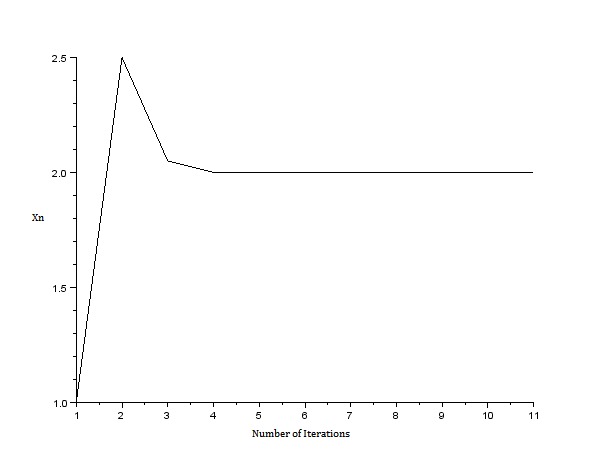
\includegraphics[width=0.4\textwidth]{10112.png}
\end{center}

\bigskip\noindent
{\bf 10.2.4 Standard Route to Chaos}\\
{\bf Solution:} \\
\noindent
{\bf 10.3.7 Decimal Shift Map}\\
{\bf Solution: }\\

{\bf a. } The Decimal Shift Map on
\begin{align*}
x_{n+1}=10x_n(mod1)
\end{align*} 
is given by the diagram below.
\begin{figure}[htp]
  \centering
  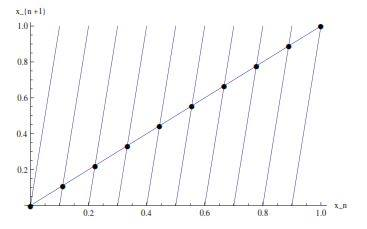
\includegraphics[width=4cm]{10_3_7_a}
  \caption{}
\end{figure}

{\bf b. } We see that all fixed points $\in [0,1]$ since for $x_n \in [o,1], x_n=0.1 p_n+0.01q_n+0.001r_n+...$ where $p_n,q_n,r_n$ are all integers then \\
\begin{align*}
x_{n+1}&=[0.1 p_n+0.01q_n+0.001r_n+...]mod1\\
&=0.1 q_n+0.01r_n+...\\
\end{align*} 
$\Rightarrow$ if we want $x_{n+1}=x_n$ then \\
\begin{align*}
p_n &=q_n\\            
q_n &=r_n \\
&\vdots\\
\Rightarrow x^* &= 0.111111...=\frac{1}{9}\\
x^*&= 0.22222...\\
x^*&= 0.3333...\\
x^*&=0.4444....\\
& \vdots \\
x^*&= 0.99999...=1
\end{align*}
which are all fixed points.\\
{\bf c. } To show that the map has periodic points, here are the periodic points are which are all unstable. \\
\begin{align*}
x_0&=0.123123123...\\
x_1&=0.231231231...\\
x_2&=0.312312312...\\
x_3&=0.123123...=x_0\\
\end{align*} 
This implies that all rational numbers are either fixed points or cycles.\\
Now, let's construct cycles of any length this way. To prove the stability of the cycle we calculate ${\pi_{x_i \in cycle}}_{\left(p numbers\right)} |f'(x_i)|= {\pi_{x_i \in cycle}}_{\left(p numbers\right)} 10 =10^p >1. \Rightarrow$ the cycles are all unstable.\\
{\bf d. } To show that the map has infinitely many periodic orbits,we note that periodic orbits correspond to $\mathbb{Q}\cap I.$ Then the periodic orbits correspond to $(\mathbb{R} \backslash \mathbb{Q})\cap I$ i.e., the set of irrational numbers in $[0,1]$ which is infinite. \\
{\bf e. } To show that the map has sensitive dependence on initial conditions, we consider the Liapunov exponent
\begin{align*}
\lambda=\lim_{n\to\infty} \frac{1}{n} \sum_{i=1}^n ln |f'(x_i)|=ln 10 
\end{align*}
$\Rightarrow$ the map is chaotic; $\forall x_0$ which is not a fixed point nor on the unstable cycle, i.e., all irrational numbers in [0,1].\\
\noindent
{\bf 10.4.9 Period Doubling in Lorenz} 
{\bf Solution:}\\
\indent
{\bf a. } \\

\noindent
{\bf 10.5.2 Lyapunov for decimal shift } \\
{\bf Solution: }\\

\bigskip\noindent
{\bf 10.6.4 Period 4}\\
{\bf Solution:}\\
{\bf a. } To show that only two patterns are possible for period -4 orbits: RLL and RLR, we refer table 1 below. Note that we are given the logistic map $x_{n+1}=rx_n(1-x_n)$ which is governed by the U- Sequence. Table 1, clearly shows that there are only two patterns which are possible for period - 4 orbits: RLL and RLR.
\begin{table}[h!]
  \centering
  \caption{U-Sequence through Period 6 (from MSS 73)}
  \label{tab:table1}
  \begin{tabular}{ccc}
    \toprule
    Period & U-Sequence & Parameter for Logistic Map\\
    \midrule
    2 & R & 3.2361\\
    4 & RLR & 3.4986\\
    6 & RLRRR & 3.6275\\
    5 & RLRR & 3.7389\\
    3 & RL & 3.8319\\
    6 & RLLRL & 3.8446\\
    5 & RLLR & 3.9057\\
    6 & RLLRR & 3.9375\\
    4 & RLL & 3.9603\\
    6 & RLLLR & 3.9778\\
    5 & RLLL & 3.9903\\
    6 & RLLLL & 3.9976\\
    \bottomrule
  \end{tabular}
\end{table}

{\bf b. } Now, table 1 also shows that period-4 orbit with pattern RLL has a value $r=3.9603$ which is larger than RLR always occurs after RLR with $r=3.4986.$\\

\bigskip

\noindent
{\bf 10.7.4 Wildness of Universal Function }\\
{\bf Solution: } To verify that the function $g(x)$ has infinitely many wiggles as $x$ ranges over the real line, we show that it crosses the line $y=\pm x$ infinitely many times by showing that if $x^*$ is a fixed point of $g(x),$ then so $ax^*.$\\  
Now, we use the universal function
\begin{align*}
g_i(x)&=\lim_{n\to\infty} a^n f^{2^n}\left(\frac{x}{a^n}, R_{n+1}\right)\\
\Rightarrow f\left(x,R_{+\infty}\right)&\approx a f^2\left(\frac{x}{a}, R_{\infty}\right)\\
\Rightarrow g(x)&=ag^2\left(\frac{x}{a}\right).
\end{align*} 
 Now, if $x^*$ is a fixed point of $g(x)$ then we have $g(x^*)=ag^2\left(\frac{x^*}{a}\right).$ Since $a$ is an arbitrary constant then it holds for any value of $a.$ Therefore, if $x^*$ is a fixed point, so is $ax^*.$ That is,$g(x^*)=ag^2\left(\frac{ax^*}{a}\right)\Rightarrow g(x^*)=ag^2\left(x^*\right)$. \mycbox{black}
\end{document}             % End of document.
